\documentclass[a4paper,12pt]{report}

\usepackage{alltt, fancyvrb, url}
\usepackage{graphicx}
\usepackage[utf8]{inputenc}
\usepackage{float}
\usepackage{hyperref}
\usepackage{listings}
\usepackage{xcolor}

% Questo commentalo se vuoi scrivere in inglese.
\usepackage[italian]{babel}

\usepackage[italian]{cleveref}

% Definizione stili per blocchi di codice
\lstdefinelanguage{bash}{
    keywords={cd, ls, mv, cp, rm, mkdir, rmdir, echo, cat, sudo, git, python3, pip, docker, npm},
    sensitive=true,
    morecomment=[l]{\#},
    alsoletter={-}
}
\lstdefinestyle{bash}{
    language=bash,
    basicstyle=\ttfamily\small,
    backgroundcolor=\color{gray!10},
    frame=single,
    breaklines=true,
    keywordstyle=\color{blue},
    commentstyle=\color{gray}\itshape,
}
\lstdefinestyle{scala}{
    language=Scala,
    basicstyle=\ttfamily\small,
    backgroundcolor=\color{gray!10},
    frame=single,
    breaklines=true,
    keywordstyle=\color{blue},
    commentstyle=\color{gray}\itshape,
    stringstyle=\color{orange},
}

\title{Relazione Assignment-03 \\
1.About Asyncronous Message Passing with Actors (not distributed)\\ per l'esame \\ ``Programmazione Concorrente e Distribuita''}
\author{Giosuè Giocondo Mainardi}

\date{\today}

\begin{document}

\maketitle

\tableofcontents

\chapter{Analisi}
% A brief analsysis of the problem, focusing in particular aspects that are relevant from concurrent point of view.
    Il modello di simulazione dei Boid, formulato da Craig Reynolds nel 1986, rappresenta un sistema multi-agente in cui 
    entità autonome (Boid) si muovono in uno spazio condiviso, modificando la propria traiettoria in funzione dei Boid 
    circostanti e di parametri predefiniti.
    
    Dal punto di vista computazionale, l'algoritmo richiede l'aggiornamento sincronizzato delle velocità di ciascun Boid 
    in base alle posizioni correnti dei vicini, seguito dall'aggiornamento delle posizioni secondo le nuove velocità 
    calcolate, per poi infine renderizzare lo stato aggiornato tramite l'interfaccia grafica.
    
    In ottica di ottimizzazione delle prestazioni tramite programmazione concorrente, emerge l'opportunità di distribuire 
    il carico computazionale tra più unità di elaborazione. Tale distribuzione deve tuttavia preservare la correttezza 
    dell'algoritmo, garantendo che l'aggiornamento delle velocità preceda sempre quello delle posizioni, e che la 
    visualizzazione avvenga solo a computazione completata.


\chapter{Design}
% A description of the adopted design, the strategy and architecture.

    % Conversione in Scala
    L'applicazione è stata completamente convertita in \texttt{Scala}, partendo dal design già sviluppato per l'Assignment-01 e adottando uno stile funzionale e pulito.

    % Architettura generale
    Il design dell'applicazione si basa su un'architettura a tre livelli, ispirata al pattern Model-View-Controller (MVC).
    \begin{itemize}
        \item \texttt{BoidsModel}: gestisce lo stato della simulazione, inclusi i Boid e le loro proprietà.
        \item \texttt{BoidsView}: si occupa della visualizzazione grafica dei Boid e dell'interfaccia utente.
        \item \texttt{BoidsSimulator}: funge da intermediario tra Model e View, gestendo la logica di aggiornamento e le interazioni dell'utente.
    \end{itemize}

    % Utilizzo Akka e adozione FSM da Dining Hakkers
    È stato poi adottato il framework \texttt{Akka} per definire un'architettura orientata al message passing, scegliendo il modello \textbf{FSM}\footnote{\href{https://doc.akka.io/libraries/akka-core/current/typed/fsm.html}{Behaviors as finite state machines}}(Finite State Machines) proposto a lezione e ispirandosi all'esempio fornito dei \texttt{Dining Hakkers}\footnote{\href{https://github.com/cric96/pcd-lab-akka-actors/blob/63e4f3273ef1550c1c744d1f7332b7ce935223ab/src/main/scala/it/unibo/pcd/akka/basics/e07fsm/DiningHakkers.scala}{Adattamento da akka-samples by cric-96}}.
    
    % Spiegazione FSM
    Utilizzando il modello \textbf{FSM}, ogni attore può essere in uno stato specifico e rispondere a messaggi in modo differente a seconda dello stato corrente, definendo diversi  \texttt{Behavior}. Questo approccio consente di gestire la logica di controllo della simulazione in modo chiaro e modulare, facilitando l'estensione e la manutenzione del codice.

    % Dove viene usato il modello FSM?
    Questo stile è stato adottato in due aree precise dell'applicazione: nell'aggiornamento dei Boids da parte del Model e nel Loop di Controllo dell'applicazione
    
    \section{Loop di Controllo dell'applicazione}
        La comunicazione nel BoidsSimulator avviene tramite due protocolli distinti:
        \begin{itemize}
            \item \texttt{Update}: per la comunicazione con il Model, gestisce i messaggi relativi all'aggiornamento dei \texttt{Boids} e della \texttt{View} 
            \item \texttt{UI}: per la gestione dell'interfaccia utente, comprende i comandi \texttt{Start}, \texttt{Stop}, \texttt{Pause}, \texttt{Resume} e \texttt{ChangeAttribute}
        \end{itemize}

        Entrambi i protocolli estendono il trait \texttt{Loop}, garantendo un'interfaccia uniforme per la gestione dei messaggi.

        Gli stati modellati nel \texttt{BoidsSimulator} sono:
        \begin{itemize}
            \item \texttt{notRunning}: lo stato iniziale.
            \item \texttt{running}: quando la simulazione è attiva e i Boids vengono aggiornati.
            \item \texttt{suspended}: quando la simulazione è sospesa, ma può essere ripresa.
            \item \texttt{start}: quando la simulazione può essere avviata correttamente.
            \item \texttt{handleAttributeChanging}: quando viene cambiato un attributo dagli sliders.
        \end{itemize}
        
    \section{Aggiornamento dei Boids}
        Nell'implementazione scelta ogni Boid è rappresentato da un attore autonomo responsabile del proprio stato e della logica di aggiornamento. Gli attori comunicano con il Model esclusivamente attraverso messaggi asincroni, garantendo una gestione naturale della concorrenza e una chiara separazione delle responsabilità.

        Il ciclo di aggiornamento dei Boids è orchestrato da un attore principale \texttt{BoidsModel} che coordina le operazioni con due semplici comandi:
        \begin{itemize}
            \item \texttt{UpdateBoidsVel}
            \item \texttt{UpdateBoidsPos}
        \end{itemize}
        Tramite questi, coordina l'aggiornamento dei singoli Boids e ne raccoglie le risposte.
        
        Ogni BoidActor, invece, può ricevere uno dei seguenti messaggi:
        \begin{itemize}
            \item \texttt{UpdateVel}: per calcolare la nuova velocità in base alle regole di interazione con i Boids vicini.
            \item \texttt{UpdatePos}: per aggiornare la posizione in base alla velocità corrente.
            \item \texttt{Kill}: per terminare l'attore Boid.
        \end{itemize}
        
\chapter{Comportamento}
% A description of the behaviour of the system using one or multiple Petri Nets, choosing the propor level of abstraction.
    % Introduzione alle reti di Petri
    Il comportamento del sistema di simulazione dei Boid viene formalizzato attraverso reti di Petri che catturano gli aspetti dinamici e la sincronizzazione tra i diversi componenti. Questo modello formale permette di rappresentare efficacemente sia l'interazione dell'utente con l'applicazione che il ciclo di aggiornamento interno della simulazione.
    Inoltre, avendo adottato il modello \textbf{FSM}, vengono forniti anche dei piccoli automi che rappresentano gli attori modellati, per evidenziare i loro possibili stati e messaggi accettabili.
    
    \section{Loop di Controllo dell'applicazione}
        Qui si descrive il flusso di controllo dell'applicazione in risposta ai comandi dell'utente.
        Una volta inizializzata l'applicazione con un numero specificato di Boid, l'utente può avviare la simulazione tramite il comando \texttt{start}. Durante l'esecuzione, è possibile fermarne completamente il funzionamento con \texttt{stop} (che riporta il sistema allo stato iniziale liberando tutte le risorse), oppure metterla temporaneamente in pausa con \texttt{suspend} per poi riprenderla successivamente con \texttt{resume}.
        \begin{figure}[ht!]
            \centering
            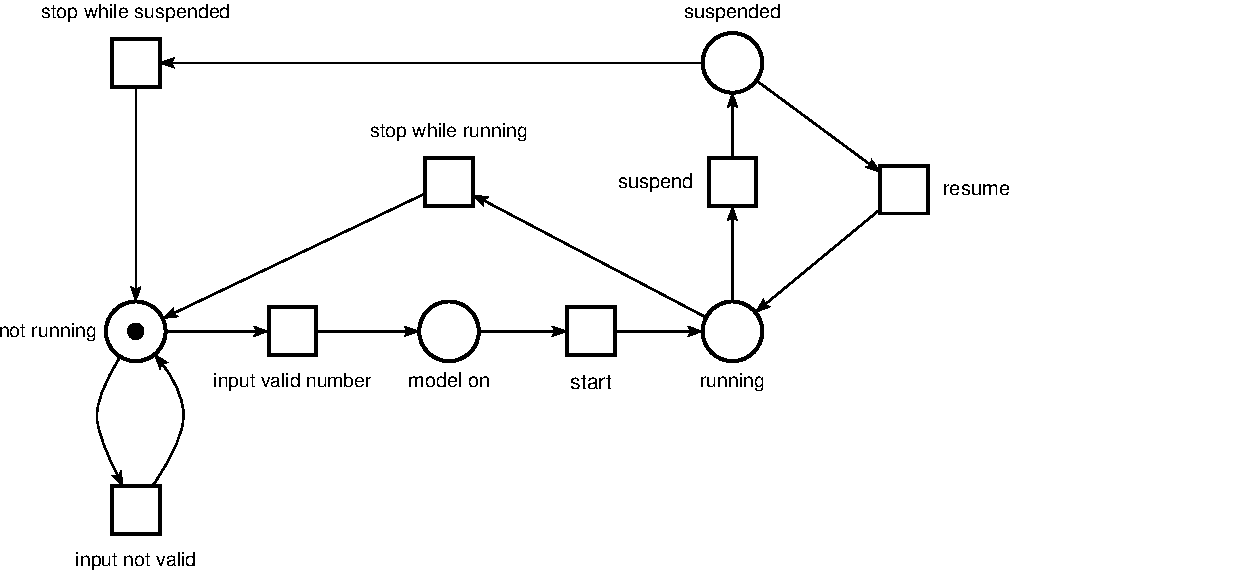
\includegraphics[width=\textwidth]{petri_nets_pdf/rete_app_flow.pdf}
            \caption{Rete di Petri per il flusso di esecuzione con input dell'utente.}
            \label{fig:rete_app_flow}
        \end{figure}
        
        Per chiarire il comportamento del comando di stop nella rete di Petri mostrata in Fig. \ref{fig:rete_app_flow}, è importante sottolineare che l'evento di stop interrompe tutti i BoidActor, senza attendere il completamento del ciclo di calcolo corrente.
        
        Questo comportamento è intenzionale e riflette l'implementazione del sistema, dove il comando di stop ha priorità assoluta e causa la terminazione immediata degli attori figli, indipendentemente dal loro stato di avanzamento nel ciclo di calcolo.

        Gli stati modellati nel \texttt{BoidsSimulator} e i possibili messaggi accettati sono rappresentati dall'automa a stati finiti (FSM) in figura:
        \begin{figure}[ht!]
            \centering
            \includegraphics[width=\textwidth]{img/FSM/Simulator.png}
            \caption{Automa a stati finiti del BoidsSimulator.}
            \label{fig:Boids_simulator_fsm}
        \end{figure}
    
    \section{Aggiornamento dei Boids}
        %ciclo di aggiornamento della simulazione, mostrando le dipendenze tra il calcolo delle velocità e l'aggiornamento delle posizioni, nonché i punti di sincronizzazione necessari per mantenere la coerenza del modello.

        Il ciclo di aggiornamento della simulazione nel Model inizia con lo stato iniziale \texttt{updateBoids}, creato dal Controller, questo passa direttamente allo stato \texttt{startUpdatingVel} che chiede a tutti i Boid di calcolare la propria velocità e si mette in attesa di risposta in \texttt{updatingVel}. Una volta che tutti i Boid hanno risposto, il Model passa allo stato \texttt{startUpdatingPos} per aggiornare le posizioni dei Boid, attende in \texttt{updatingPos} fino a quando tutti i Boid hanno aggiornato le loro posizioni. 
        Infine, dopo aver ricevuto tutte le risposte, il Model passa allo stato \texttt{endUpdatingPos} che dice al Controller di aggiornare la View, poi termina.
                
        \begin{figure}[ht!]
            \centering
            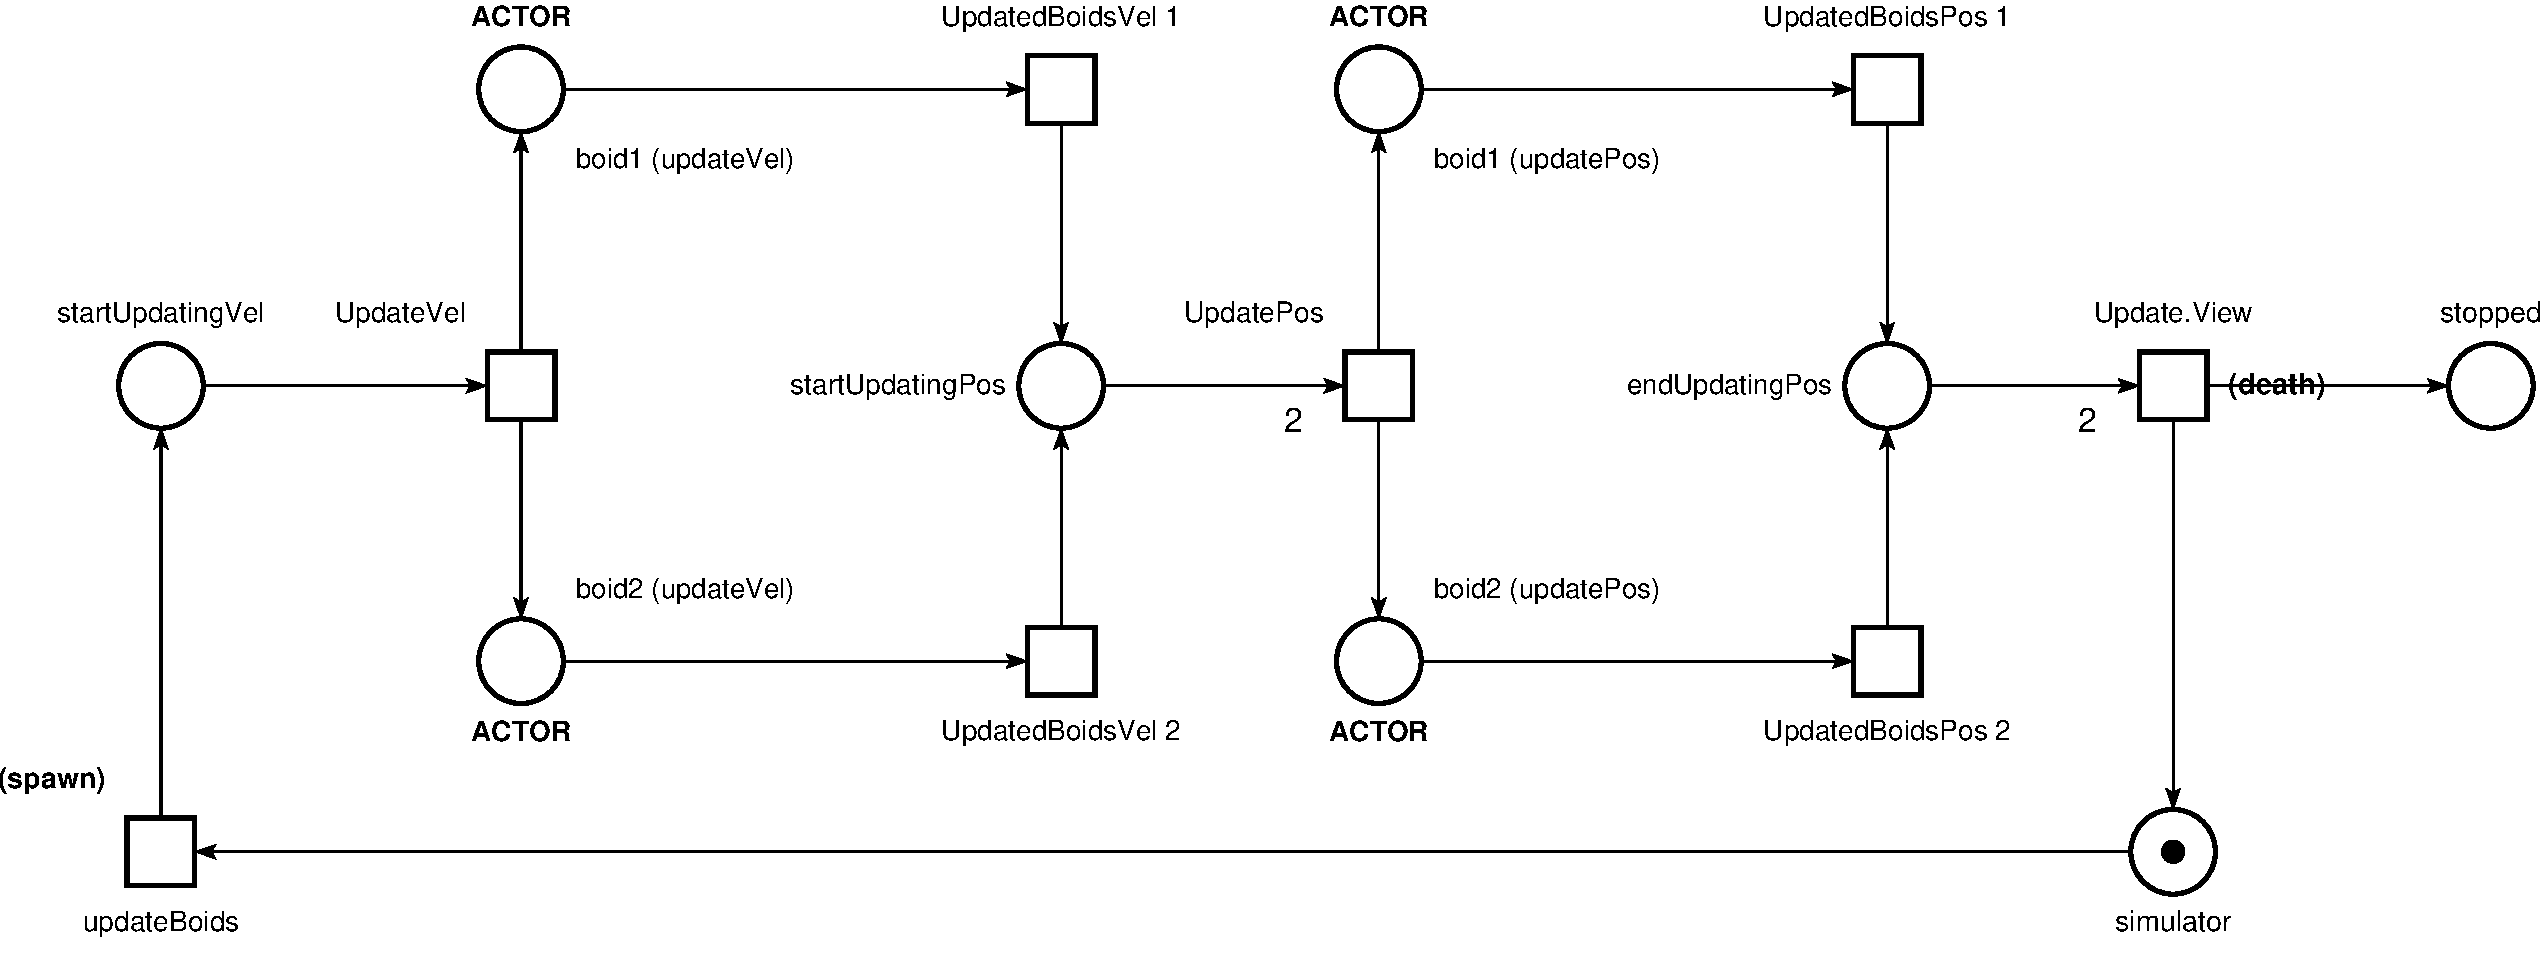
\includegraphics[width=0.8\textwidth]{petri_nets_pdf/rete_update_cycle.pdf}
            \caption{Rete di Petri per il ciclo di aggiornamento della simulazione.}
            \label{fig:rete_update_cycle}
        \end{figure}
        
        Questa rete evidenzia chiaramente i punti di sincronizzazione necessari per mantenere la coerenza del modello, garantendo che le operazioni di calcolo delle velocità e aggiornamento delle posizioni siano eseguite in modo sequenziale e coordinato tra i vari BoidActors.

        Per migliorare la comprensione del ciclo di aggiornamento della simulazione, è stato creato un automa a stati finiti (FSM) che rappresenta il comportamento del Model. Questo automa mostra gli stati principali e le transizioni tra di essi, modellati con messaggi.

        \begin{figure}[ht!]
            \centering
            \includegraphics[width=\textwidth]{img/FSM/BoidsModel.png}
            \caption{Automa a stati finiti del BoidsModel.}
            \label{fig:Boids_model_fsm}
        \end{figure}

        Ogni BoidActor può aggiornare il suo stato tramite i messaggi \texttt{UpdateVel} e \texttt{UpdatePos}, oppure terminare la propria esecuzione con il messaggio \texttt{Kill}. Questi messaggi sono gestiti in modo asincrono, consentendo a ciascun BoidActor di operare in parallelo con gli altri.

        Il suo automa può essere rappresentato come in figura:
        \begin{figure}[ht!]
            \centering
            \includegraphics[width=\textwidth]{img/FSM/BoidActor.png}
            \caption{Automa a stati finiti del BoidActor.}
            \label{fig:Boid_actor_fsm}
        \end{figure}

        \begin{lstlisting}[style=bash, caption={Avvio dello script}]
            $ mvn clean javafx:run
        \end{lstlisting}
    
    
\end{document}
